\section{Ejercicios}

\subsection{Ejercicio 1: TaskConsola}
En este ejercicio, debimos programar una tarea \textit{TaskConsola}, la cual debe realizar $n$ llamadas bloqueantes, cada una con 
una duraci\'on al azar entre los n\'umeros $bmin$ y $bmax$, que la tarea recibir\'a como par\'ametro.

Para ello, decidimos generar, $n$ veces, un n\'umero pseudo-aleatorio por medio de la 
funci\'on \textit{rand()} (devolver\'a un n\'umero aleatorio entre 0 y 1) y luego, mediante la f\'ormula:

\begin{verbatim}
 random = b_min + (rand() % (int)(b_max-b_min+1));
\end{verbatim}

tendremos un n\'umero aleatorio en el rango deseado. 
Luego, para cada n\'umero aleatorio generador, realizamos una llamada bloqueante (uso\_IO) 
que durar\'a tantos ciclos de clock como indique el n\'umero aleatorio generado.

\subsection{Ejercicio 2: Experimentando FCFS}
Para probar el Scheduler First Came First Served, usaremos el siguiente lote de tareas:

\begin{verbatim}
  TaskCPU 10
  TaskConsola 5 1 5
  TaskConsola 3 1 2
\end{verbatim}

En la primera, utlizaremos TaskCPU y, para simular el uso intensivo, correr\'a durante 10 ciclos de reloj.
Las siguientes tareas son del tipo TaskConsola implementado anteriormente, pas\'andole como par\'ametro el n\'umero de llamadas 
bloqueantes y el rango en el cual debe seleccionar el n\'umero aleatorio.

En el algoritmo FCFS, la CPU se asigna a los procesos en el orden en que son solicitan.\\
Por lo tanto, esperamos observar que, con un solo n\'ucleo, un proceso no pueda correr 
hasta que no terminaron los anteriores a \'el.

Por otro lado, al correr la simulaci\'on con dos nucleos, correr\'an dos procesos simlt\'aneamente y el tercero empezar\'a cuando alguno de los otros 
dos finalice y, por \'ultimo, si el procesador tiene 3 n\'ucleos, los 3 correr\'an en simult\'aneo, uno en cada n\'ucleo.

\vspace{\baselineskip}
\begin{center}
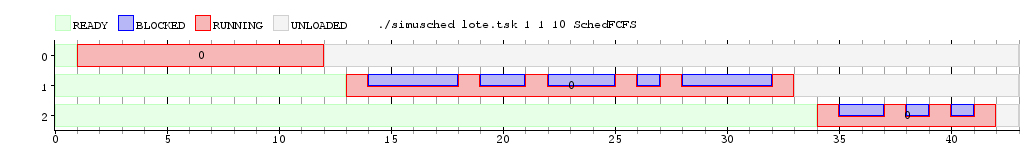
\includegraphics[scale=0.45]{../tp1/Test/resEj2Co1.png}
\\
\vspace{1pt}
\footnotesize\textit{Simulacro FCFS con un n\'ucleo}
\end{center}
\vspace{\baselineskip}


\vspace{\baselineskip}
\begin{center}
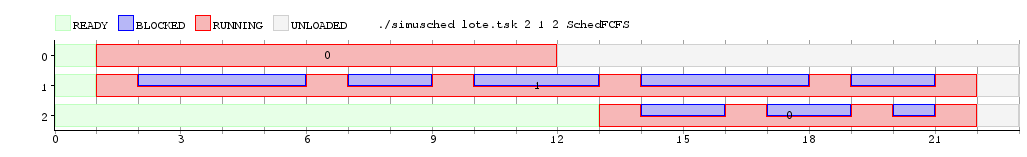
\includegraphics[scale=0.45]{../tp1/Test/resEj2Co2.png}
\\
\vspace{1pt}
\footnotesize\textit{Simulacro FCFS con dos n\'ucleos}
\end{center}
\vspace{\baselineskip}

\vspace{\baselineskip}
\begin{center}
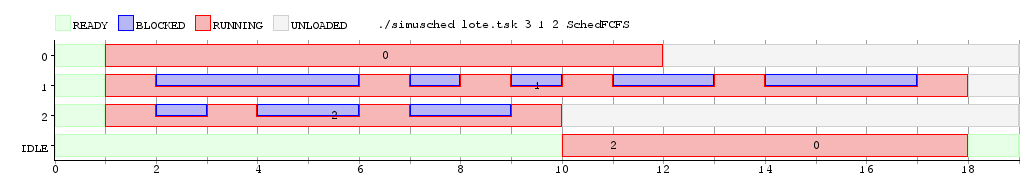
\includegraphics[scale=0.45]{../tp1/Test/resEj2Co3.png}
\\
\vspace{1pt}
\footnotesize\textit{Simulacro FCFS con tres n\'ucleos}
\end{center}
\vspace{\baselineskip}


Los experimentos corroboraron nuestra hip\'otesis, pues el comportamiento reflejado es exactamente el descripto previamente.

Adem\'as, notemos que en los casos en los que utilizamos la tarea TaskConsola, se observan claramente
las llamadas bloqueantes de manera aleatoria, dado que el tiempo tanto de la ejecuci\'on como el de las llamadas bloqueantes var\'ia.
En el caso en que el procesador tiene tres n\'ucleos, se observa que los n\'ucleos 2 y 0 ejecutan la tarea
Idle, ya que est\'an desocupados, esperando la solicitud del pr\'oximo proceso.

\subsection{Ejercicio 3: Implementando Round-Robin}
La idea del scheduler \textit{Round-Robin} es asignarle un quantum a cada procesador y luego, ir iterando los procesos, 
para que todos ejecuten una vez (durante el quantum que le fue asignado al procesador, o menos, en caso de que terminen
o se bloqueen antes) antes de volver a comenzar la iteraci\'on.

Con esta idea desarrollamos nuestro Scheduler Round-Robin. Utilizamos como estructura una cola $(q)$ para almacenar los \verb|id| de los procesos, 
un vector $(quantum)$ con tantas posiciones como cantidad de cores, que almacenar\'a el quantum del i\'esimo n\'ucleo, 
y otro vector $(contador)$ que va a llevar cuenta del tiempo corrido por el proceso en el i\'esimo n\'ucleo hasta llegar al quantum del mismo.

Para el correcto funcionamiento de la funci\'on $tick$ se ven reflejados los casos en el cual el proceso debe 
dejar de correr, ya sea porque termin\'o su ejecuci\'on o el quantum del procesador en el que corr\'ia se agot\'o. En \'este \'ultimo 
caso, la posici\'on correspondiente al n\'ucleo en $contador$ volver\'a a cero y el proceso se encolar\'a para terminar con su tiempo en la pr\'oxima vuelta. 
\\Una vez realizada dicha acci\'on, debe dar lugar a la siguiente en la cola. En caso de no haber una, se ejecutara la tarea IDLE hasta el llamado de una 
nueva tarea.

\subsection{Ejercicio 4: Experimentando Round-Robin}

En este ejercicio nos proponemos experimentar con el scheduler del punto anterior para verificar que el comportamiento es el esperado. Haremos esto de 
manera incremental, es decir, empezaremos probando las cosas mas b\'asicas e iremos subiendo la complejidad. 

Para empezar, probaremos Round Robin con un solo n\'ucleo. N\'otese que si le asignamos una sola tarea, su comportamiento no diferir\'ia de cualquier otro 
scheduler, por lo que empezamos probando con un lote con cuatro tareas. Estas tareas s\'olo usar\'an el cpu, es decir, no har\'an llamadas bloqueantes.
Esperamos verificar que el scheduler Round Robin le asigna el tiempo del quantum a cada tarea antes de comenzar de nuevo a iterar la lista de tareas
pendientes.

\vspace{\baselineskip}
\begin{center}
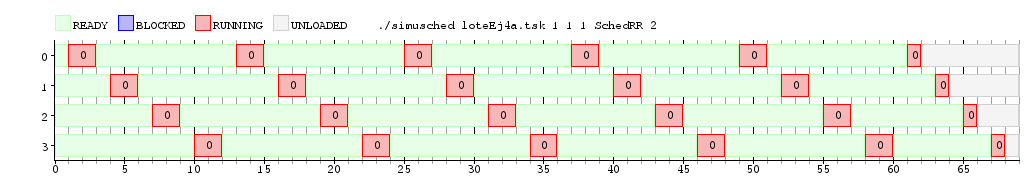
\includegraphics[scale=0.45]{../tp1/Test/resEj4Co1SB.png}
\\
\vspace{1pt}
\footnotesize\textit{Simulacro RR con un n\'ucleo}
\end{center}
\vspace{\baselineskip}

Efectivamente, cuando recibe $k$ tareas, el scheduler le asigna tiempo de ejecuci\'on a las tareas de modo que todas 
ejecuten antes de regresar a ejecutar la primera. 

A continuaci\'on, usaremos el mismo lote de tareas, pero agregaremos otro procesador. As\'i, veremos si el scheduler maneja correctamente 
los procesadores para asegurarse que todas las tareas ejecuten un tiempo $quantum$ antes de volver a empezar.

\vspace{\baselineskip}
\begin{center}
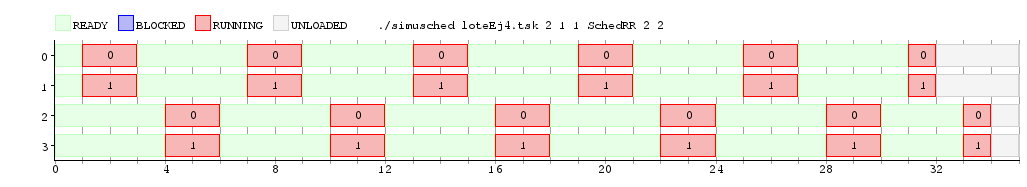
\includegraphics[scale=0.45]{../tp1/Test/resEj4Co2SB.png}
\\
\vspace{1pt}
\footnotesize\textit{Simulacro RR con dos n\'ucleo}
\end{center}
\vspace{\baselineskip}

El comportamiento es id\'entico al anterior, s\'olo que agregando otro nucleo, es decir, podemos deducir las mismas conclusiones. Para probar de 
modo mas realista este scheduler, simularemos un lote de cuatro tareas que realicen llamadas bloqueantes, con dos procesadores para su ejecuci\'on.
Lo que queremos mostrar, es que el scheduler trabajara de manera \'optima en este caso, no d\'andole tiempo de CPU a una tarea bloqueada.

\vspace{\baselineskip}
\begin{center}
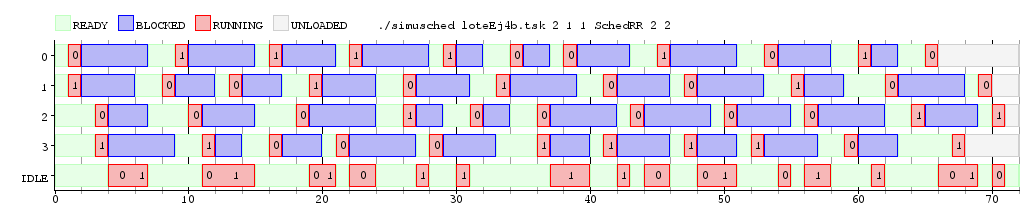
\includegraphics[scale=0.45]{../tp1/Test/resEj4Co2CB.png}
\\
\vspace{1pt}
\footnotesize\textit{Simulacro RR con dos n\'ucleo}
\end{center}
\vspace{\baselineskip}

Podemos ver que el scheduler trabaja de la manera esperada. Es decir, si hay un tarea disponible para ejecutar y procesador que no esta ejecutando nada,
ese procesador carga la tarea y la ejecuta, o bien hasta que se le acabe el quantum o hasta que se bloquee. Si todas las tareas estan bloqueadas 
o ejecutando cuando el procesador termina la ejecucion de una tarea porque se bloqueo, este se poner a ejecutar la tarea IDLE hasta que 
una tarea se desbloque. Y por lo tanto, si todas las tareas estan bloqueadas, ambos procesadores ejecutan la tarea IDLE hasta que alguna 
tarea se desbloquee.


\subsection{Ejercicio 5: \textit{Scheduling algorithms for multiprogramming in a hard-real-time environment}}
Este ejercicio est\'a dividido en dos incisos: en el primero, contestaremos una serie de preguntas formuladas por la c\'atedra, basando nuestras respuestas en el 
art\'iculo \textit{Scheduling algorithms for multiprogramming in a hard-real-time environment}; en el segundo, explicaremos el dise\~no e implementaci\'on 
de los algoritmos de scheduling de prioridades fijas y din\'amicas presentados en dicho art\'iculo.
\subsection*{Inciso 1}
En este inciso, debemos contestar tres preguntas te\'oricas acerca de los algoritmos de scheduling propuestos en el art\'iculo previamente mencionado. Antes de 
contestar las preguntas, comenzaremos con una breve descripci\'on de las condiciones de entorno sobre las cuales los algoritmos fueron ideados.
\newline
\newline
Se cuenta con un sistema, con un conjunto de tareas destinadas a resolver, cada una, una determinada funcionalidad vital para el correcto funcionamiento
de dicho sistema. Cada una de estas tareas estar\'a asociada a un evento externo, que solicitar\'a su ejecuci\'on. Es importante destacar que las tareas no
pueden ser ejecutadas antes de que dicho evento las solicite. Adem\'as, se sabe que cada tarea tiene, por un lado, una \textit{deadline} (esto es, una cantidad
de tiempo m\'aximo en el cual su ejecuci\'on debe terminar), que se mantendr\'a constante durante toda la ejecuci\'on del sistema. Por otro lado, se sabe
que el evento que solicitar\'a la ejecuci\'on de cada tarea, solicitar\'a peri\'odicamente (esto es, el intervalo de tiempo entre dos solicitudes ser\'a
siempre el mismo y no depender\'a de la terminaci\'on de otras tareas solicitadas) la ejecuci\'on de dicha tarea y, adicionalmente, se sabe que el tiempo de 
ejecuci\'on de cada tarea (entendiendo tiempo de ejecuci\'on como la cantidad de clocks que le llevar\'ia a una tarea comenzar y terminar su ejecuci\'on si el 
procesador s\'olo tuviera que ejecutar a esa tarea) ser\'a constante. Una condici\'on extra establece la existencia de tareas no peri\'odicas: estas tareas
desplazaran del procesador a las peri\'odicas y, a diferencia de las peri\'odicas, no tendr\'an una deadline estricta para terminar. Una vez establecidas
las condiciones del sistema, estamos listos para contestar las preguntas:
\newline
\newline
\textit{a}) \textquestiondown Qu\'e problema est\'an intentando resolver los autores?
\newline
\newline
Dado un sistema que se ajuste a las condiciones de entorno previamente explicadas, los autores quieren hallar una forma heur\'istica de organizar la ejecuci\'on de las
tareas, a medida que estas son solicitadas, de manera tal de que todas terminen su ejecuci\'on antes de su respectiva \textit{deadline}. Para esto, los 
algoritmos presentados estar\'an basados en prioridades, es decir, c\'omo se le asignar\'a la prioridad a cada tarea variar\'a seg\'un el algoritmo. Luego, los algoritmos
de scheduling deber\'an desalojar a la tarea que est\'e ocupando el procesador si llega una solicitud para la ejecuci\'on de una
tarea m\'as prioritaria. Por lo tanto, la clave para este tipo de algoritmos estar\'a en c\'omo se le asignar\'an las prioridades a las tareas.
\newline
\newline
\textit{b}) \textquestiondown Por qu\'e introducen el algoritmo de la secci\'on 7? \textquestiondown Qu\'e problema buscan resolver con esto?
\newline
\newline
Los autores introducen el algoritmo de la secci\'on 7, buscando bajar la cota superior de \verb|ln 2| sobre el tiempo de utilizaci\'on del procesador establecida 
por el algoritmo de scheduling con prioridades fijas, sin tener que asumir ninguna hip\'otesis extra para los tiempos de ejecuci\'on de las tareas, ni tampoco 
necesitar relajar las \textit{deadlines} de las tareas menos prioritarias seg\'un el esquema anterior. Para lograr esto, introducen el algoritmo de 
scheduling con prioridades asignadas din\'amicamente; es decir, a lo largo de la ejecuci\'on del sistema, las prioridades de las tareas no estar\'an
necesariamente fijas.
\newline
\newline
\textit{c}) Explicar coloquialmente el significado del teorema 7.
\newline
\newline
El teorema 7 establece una condici\'on necesaria y suficiente, sobre el algoritmo de prioridades din\'amicas, para que todas las tareas terminen de ejecutarse
antes de su \textit{deadline}. Dicha condici\'on es la siguiente:

\begin{equation*}
 C_{1}/T_{1} + ... + C_{n}/T_{n} \leq 1
\end{equation*}

donde
\begin{itemize}
  \item $n:=$ n\'umero de tareas en el sistema
  \item $C_{i}:=$ tiempo de ejecuci\'on de la tarea i\'esima
  \item $T_{i}:=$ tiempo entre dos solicitudes consecutivas por la tarea i\'esima (tambi\'en llamado per\'iodo)
\end{itemize}

Es importante se\~nalar que la condici\'on que establece este teorema nos permitir\'a, dado un lote de tareas dise\~nado para nuestros experimentos, definir 
si el algoritmo de scheduling con propiedades din\'amicas lograr\'a que todas las tareas terminen de ejecutar antes de sus respectivas \textit{deadlines}, a lo 
largo de toda la simulaci\'on.

\subsection*{Inciso 2}

En este inciso explicaremos brevemente en qu\'e consiste cada algoritmo de scheduling, y luego el dise\~no y la implementaci\'on de cada uno.

Como su nombre indica, el algoritmo de scheduling con prioridades fijas le asignar\'a a las tareas una prioridad que se mantendr\'a fija a lo largo de 
toda la ejecuci\'on del sistema. Concretamente, una tarea ser\'a m\'as prioritaria que otra cuando su per\'iodo, l\'ease el tiempo constante transcurrido entre
dos solicitudes por dicha tarea, sea el menor de los dos. O equivalente, que su \textit{request rate}, definido como el inverso multiplicativo del per\'iodo,
sea mayor. 

Para el dise\~no de este algoritmo de scheduling, optamos por utilizar una cola de prioridad, que contendra duplas de la forma 
$<periodo(pid),pid>$, donde el m\'as prioritario ser\'a el que tenga menor per\'iodo. Este dise\~no nos permitir\'a obtener de manera sencilla cu\'al es
la pr\'oxima tarea a ser ejecutada, aprovechando las funcionalidades ya implementadas en la clase \textit{priority queue} para encolar elementos y obtener
el m\'as prioritario. De esta manera, obtener en cada tick de reloj cu\'al es la tarea a ejecutarse se resumir\'a a verificar, en primer lugar, si la 
cola de prioridad est\'a vac\'ia. En caso de que est\'e vac\'ia, se ejecutar\'a la tarea IDLE; en caso contrario, se obtendr\'a el \textit{pid} de la 
pr\'{o}xima tarea a ser ejecutada mediante la funci\'on \textit{top()}, devolviendo el segundo componente de la dupla devuelta por dicha funci\'on.

A diferencia del algoritmo anterior, el algoritmo de scheduling con prioridades din\'amicas, le asignar\'a las prioridades a cada tarea en cada
\textit{tick} de reloj. Esto se hara de la siguiente manera: a cada momento de la ejecuci\'on del sistema, la tarea m\'as prioritaria ser\'a la que
tenga su \textit{deadline} m\'as pr\'oxima; coloquialmente, esto quiere decir que lo m\'as urgente ser\'a lo m\'as prioritario. Para el dise\~no de
este scheduler, como deb\'iamos actualizar las prioridades en todos los \textit{ticks} de reloj, optamos por utilizar arreglos en vez de una cola de 
prioridad. Esto es porque, de utilizar una cola de prioridad, ser\'ia m\'as complicado iterar los procesos contenidos en la tabla para actualizar sus prioridades.
Por lo tanto, contaremos con los siguientes arreglos:

\begin{itemize}
  \item \textit{int deadline[totaltasks]} indicara, para la tarea i\'esima, cu\'anto tiempo le queda antes de su \textit{deadline} en $deadline[i]$. Para las tareas
  no peri\'odicas, adoptamos la convenci\'on de almacenar un -1 en esa posici\'on del arreglo.
  \item \textit{bool ready[total tasks]} indicar\'a, para la tarea i\'esima, si est\'a lista para correr o no.
\end{itemize}

Adicionalmente, implementamos la funcion \textit{int tareasready()}, que devolver\'a la cantidad de tareas en estado \textit{ready}.
Para obtener, en cada \textit{tick} de reloj, la pr\'oxima tarea a ejecutarse, implementamos una funci\'on de acuerdo a la siguiente l\'ogica:
Si est\'a corriendo una tarea no peri\'odica, seguir ejecutando esa. En caso contrario, verificar, en primer lugar, si hay alguna tarea
no peri\'odica en estado \textit{ready}. En caso de haberla, pasar a ejecutar esa; en caso contrario, buscar la tarea peri\'odica en estado
\textit{ready} cuya \textit{deadline} est\'e m\'as pr\'oxima y devolver esa. Vale la pena aclarar
que adem\'as, en cada \textit{tick} de reloj, se decrementar\'a el valor contenido en el arreglo \textit{deadline} para cada tarea peri\'odica que est\'e
lista para ejecutarse. En este punto, hacemos la aclaraci\'on de que hemos dejado fuera de la descripci\'on algunos de los casos borde para los cuales no 
haya tareas listas para ejecutarse, en que deba devolverse el \textit{pid} de la tarea Idle, ya que no suma a la comprensi\'on del caso en que el algoritmo
deba buscar, entre las tareas existentes, la m\'as prioritaria.

\subsection{Ejercicio 6: TaskBatch}

En este ejercicio implementamos la tarea TaskBatch, que recibe como parametros \verb|totalcpu| y \verb|cantbloqueos|. Esta tarea dura, en total, \verb|totalcpu| 
ciclos de clock, y realiza \verb|cantbloqueos| llamadas bloqueantes en momentos psudoaleatorios. Implementamos esta tarea de dos maneras. La primera implementaci\'on itera totalcpu
veces pidiendo un numero aleatorio rand. Si rand > 0.5, entonces har\'a una llamada bloqueante, sino, a una tarea que use el cpu. Si la cantidad 
de iteraciones se acaba sin haber realizado todas las llamadas bloqueantes, entonces se realizaban las restantes seguidas al final. Sino, cuando se realizaba
la ultima llamada bloqueante, se utilizaba el tiempo restante del cpu todo junto. Lo que observamos en esta implementacion fue que las llamadas bloqueantes
se hacian para tiempos grandes siempre al principio del intervalo de uso del cpu, y para tiempos de medianos a cortos, siempre al final.

Por eso realizamos otra implementacion. En esta se seleccionan previamente en que momentos se van a realizar las llamadas bloqueantes, marcando en un arreglo de \verb|totalcpu| 
posiciones los momentos en los que se va a llamar la tarea bloqueante. Se decide los momentos de bloqueo eligiendo un numero aleatorio entre 0 y totalcpu, 
asegurandonos de que no halla repetido. 
Finalmente, iteramos este arreglo y llamamos a UsoIO si debemos hacer un bloqueo y a Uso CPU (pas\'andole 1 ciclo de clock por par\'ametro) en caso contrario.

\subsection{Ejercicio 7}
En el siguiente ejercicio, se nos pide escoger distintas m\'etricas para poder analizar el rendimiento del Shcheduler Round Robin para tareas de tipo TaskBatch.\\
A continuaci\'on, daremos algunos detalles de las mismas\\

\textbf{\underline{Fariness}}\\
Medimos que cada proceso reciba una dosis "justa" de CPU. Es decir, todos los procesos deben correr la misma cantidad de tiempo; en el caso de Round Robin, podemos decir el quantum que se le asigna a los procesos sea el mismo en todos los casos.\\

\textbf{\underline{Tiempo de Respuesta}}\\
En este caso, ser\'ia el tiempo que tarda una tarea en empezar a ejecutarse.
Cuanto tiempo permanece en estado ready hasta la primera ejecucion.\\
En el caso de Round Robin, esto depende de cu\'antas tareas hay esperando antes de la misma, ya que en este Scheduler se utiliza una cola como estructura, y ademas de cuantos n\'ucleos tiene el procesador.\\

\textbf{\underline{Throughput}}\\
Son la cantidad de procesos que terminan por unidad de tiempo.\\
Esto depender\'a de la cantidad de bloqueos que tenga cada proceso y como se organiza la CPU en cuanto a quantum y cantidad de n\'ucleos.\\

\textbf{\underline{Turnaround}}\\
Es el tiempo total que le toma a un proceso su ejecuci\'on completa, contando bloqueos y cantidad de corridas en quantums de alg\'un n\'ucleo del CPU.\\

Para este ejercicio escogimos las m\'etricas \textit{Tiempo de Respuesta} y \textit{Turnaround}

Para empezar, tomaremos una arquitectura con un solo n\'ucleo y con un quantum de 3 clocks.\\
\vspace{\baselineskip}
\begin{center}
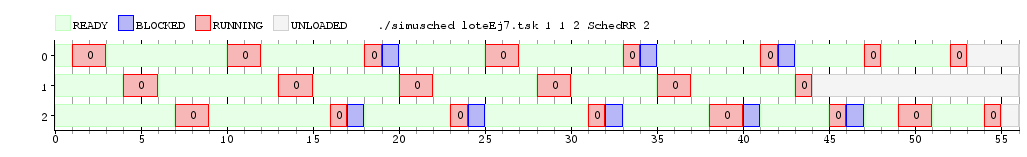
\includegraphics[scale=0.45]{../tp1/Test/resEj7Co1.png}
\\
\vspace{1pt}
\footnotesize\textit{Simulacro RR con un n\'ucleo de quantum 2}
\end{center}
\vspace{\baselineskip}


\textit{Tiempo de Respuesta}\\
Para esta m\'etrica el Scheduler no es \'optimo ya que, en nuestro experimento, al tener un solo n\'ucleo, cada proceso va a tener que esperar el comienzo de los anteriores en la cola, por lo tanto estar\'a m\'as tiempo en estado ready esperando comenzar la ejecuci\'on.\\
\textit{Turnaround}\\
Al igual que la m\'etrica estudiada anteriormente, el tiempo de respuesta influye en esta medida, ya que el proceso va a demorar en comenzar. \\
Otro factor que influye en esto es el quantum y la cantidad de n\'ucleos que tiene el procesador, ya que pudimos ver que al tener poco no es lo suficientemente bueno.Por eso nos preguntamos que pasar\'ia si los aumentamos.\\
De esta manera pueden suceder dos cosas: la primera, que tengan la misma cantidad de quantum ambos n\'ucleos y, la segunda, que sean distintos.
A continuaci\'on, estudiaremos ambos casos.\\
\vspace{\baselineskip}
\begin{center}
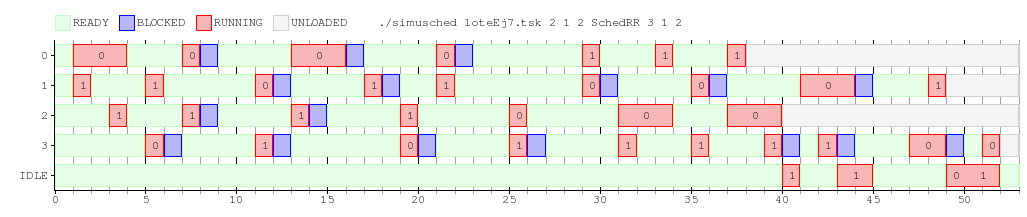
\includegraphics[scale=0.45]{../tp1/Test/resEj7Co2.png}
\\
\vspace{1pt}
\footnotesize\textit{Simulacro RR con dos n\'ucleos de quantum iguales a 2}
\end{center}
\vspace{\baselineskip}

Si nos basamos en la teor\'ia, podemos decir que cuando el Scheduler corre con dos n\'ucleos, el \textit{Tiempo de Respuesta} va a mejorar en comparaci\'on al procesador con un n\'ucleo, ya que hay uno m\'as que puede ser utlizado, lo cual disminuye el tiempo en que un proceso debe esperar en ready.\\
Utilizando como m\'etrica \textit{Turnaround}, concluimos que la mejora con respecto al primer experimento es que adem\'as de que alg\'un proceso comenzar\'a a ejecutarse antes, ya que ahora hay un n\'ucleo m\'as, al suceder esto tambi\'en tiene menos tiempo de espera entre corridas, el cual puede variar seg\'un el tiempo de migraci\'on de cada n\'ucleo.


\vspace{\baselineskip}
\begin{center}
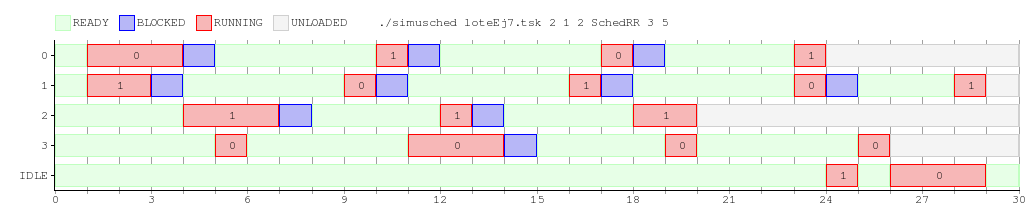
\includegraphics[scale=0.45]{../tp1/Test/resEj7Co2dis.png}
\\
\vspace{1pt}
\footnotesize\textit{Simulacro RR con dos n\'ucleos de quantum distintos}
\end{center}
\vspace{\baselineskip}

Luego, en el caso de tener quantum distintos, el \textit{Tiempo de Respuesta} no difiere demasiado del caso de tener iguales. Esto puede variar seg\'un la distribuci\'on de los quantum en los n\'ucleos, ya que en el caso de tener uno muy grande y otro muy chico, el primero estar\'a ocupado mucho tiempo, lo cual ser\'ia equivalente a tener uno solo con un tiempo peque\~no.\\
Podemos notar diferencias en \textit{Turnaround}: la mejora con respecto al anterior es que el proceso que sea beneficiado con el n\'ucleo con mayor quantum tiene posibilidades de terminar antes.


\vspace{0,5 cm}
Podemos concluir con estos experimentos que, deducir que si un Scheduler es mejor var\'ia seg\'un algunos factores y que m\'etrica estemos utilizando.\\
Pudimos ver que \textit{Tiempo de Respuesta} var\'ia segun la cantidad de n\'ucleos y, de tener distintos quantums, esto puede mejorar los resultados.\\
Para \textit{Turnaround} depende de varias cosas: en caso de que los quantums sean iguales, la mejora se encuentra en que tenemos un n\'ucleo mas y el proceso tendra m\'as chances para comenzar su ejecuci\'on, pero si tenemos distintos podemos obtener resultados a\'un mas satifactorios, seg\'un el proceso que resulte beneficiado.\\
Si ampliamos nuestro experimento a un caso con muchos procesos y n\'cleos la m\'etrica m\'as adecuada para obtener resultados satifactorios ser\'a \textit{Turnaround}, pues teniendo distintos quantums los procesos beneficiados ser\'an a\'un m\'as. \\
Si bien el \textit{Tiempo de Respuesta} va a mejorar, si se tienen muchos procesos, a\'un teniendo muchos procesadores los que se encuentren en la cola van a tener que esprar a que los mismos sean desocupados.

\subsection{Ejercicio 8: Round Robin sin migraci\'on}

En este ejercicio implementamos una nueva versi\'on del scheduler Round Robin, llamada RoundRobin2, cuya diferencia con la implementaci\'on original
es que no permite migraciones de procesos entre n\'ucleos. En primer lugar, detallaremos las estructuras de datos utilizadas para el dise\~no de
este scheduler, y luego pasaremos a mostrar los resultados de nuestra experimentaci\'on.

Para el dise\~no del scheduler, decidimos utilizar un arreglo de colas (con tantas posiciones como procesadores haya) y un arreglo de contadores de la misma 
longitud. La cola i\'esima del arreglo contendr\'a los process id de las tareas asignadas a dicho procesador, mientras que el contador i\'esimo tendr\'a un 
valor correspondiente a cu\'antas tareas hay activas en dicho procesador. Teniendo estas estructuras de datos, la asignaci\'on de una tarea a un cpu consistir\'a
en recorrer el arreglo de contadores y devolver el \'indice de alguno de los que tenga valor m\'inimo. 
Adicionalmente, contaremos con una lista de pares de la forma $<pid,cpu>$, para guardar informaci\'on sobre las tareas bloqueadas de la siguiente manera: 
cada vez que una tarea se bloquee, almacenaremos una dupla de esa manera, para saber a qu\'e procesador estaba asignada. Cuando dicha tarea se desbloquee,
bastar\'a con buscarla en la lista de pares, obtener el $cpu$ al que estaba asignada previamente, y volverla a encolar en la cola correspondiente, evitando
as\'i la migraci\'on entre n\'ucleos.

Contando con estas estructuras tendremos, mirando individualmente a cada procesador, un funcionamiento an\'alogo al de la primera implementaci\'on
de Round Robin, es decir, un recorrido circular por las tareas, con un quantum m\'aximo en que las tareas podr\'an ejecutarse.

Ahora pasaremos a comparar esta versi\'on del scheduler Round Robin con la presentada en el ejercicio 3. Estas implementaciones exhibir\'an comportamientos 
diferentes solo en determinados casos, que ser\'an los usaremos como ejemplos, mientras que las similitudes entre los comportamientos de las dos pol\'iticas
de scheduling ser\'an dejados de lado en nuestro an\'alisis (por ejemplo, la rotacion total de 
las tareas). Por lo tanto, compararemos la eficiencia en el uso de los procesadores, para lo cual usaremos como indicador la cantidad de tiempo de cpu 
utilizado en cada una de las implementaciones.
Para esto, correremos con dos procesadores el siguiente lote de tareas:

\begin{verbatim}
    TaskCPU 10
    TaskCPU 5
    TaskCPU 20
\end{verbatim}

 La idea ser\'a comparar cu\'anto tarda cada scheduler en completar el procesamiento total. N\'otese que creamos este caso ubicando 
 intencionadamente la tarea de menor ejecuci\'on en el medio. Esto forzar\'a al RoundRobin2 a usar uno de los procesadores 
 para ejecutar \'unicamente una tarea corta, mientras que deber\'a usar el otro para dos tareas temporalmente m\'as costosas.
 Es decir, mediante este lote de tareas, estamos representando en general a aquellos casos en que la asignaci\'on de los procesadores 
 para las tareas sea poco equitativa (el cual, por otro lado, es un escenario perfectamente posible, pues el scheduler no tiene porqu\'e
 saber cu\'an costosas ser\'an las tareas a ejecutar). Adicionalmente, se debe tener en cuenta que el costo de migracion 
 es de 2 ticks de reloj, el cual es un costo relativamente bajo teniendo en cuenta que, en un procesador real, migrar entre procesadores
 llevar\'ia a invalidar algunas memoias cach\'e, lo cual afectar\'ia m\'as significativamente el rendimiento.

\vspace{\baselineskip}
\begin{center}
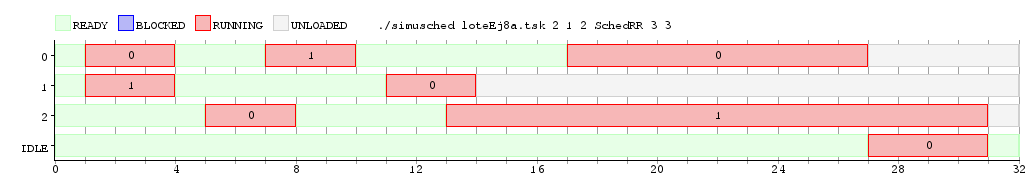
\includegraphics[scale=0.45]{../tp1/Test/resEj8Co2SBRR.png}
\\
\vspace{1pt}
\footnotesize\textit{Simulacro RR con 2 n\'ucleos de quantum 3.\\CCon costo de migracion de 2 ticks.}
\end{center}
\vspace{\baselineskip}

\vspace{\baselineskip}
\begin{center}
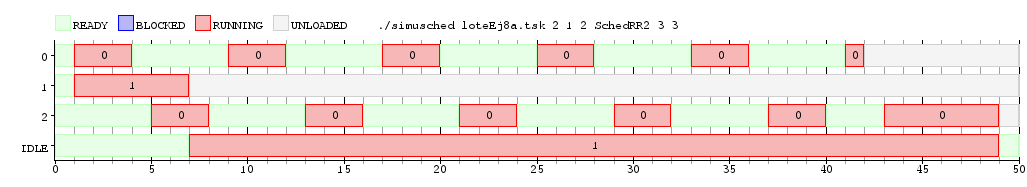
\includegraphics[scale=0.45]{../tp1/Test/resEj8Co2SBRR2.png}
\\
\vspace{1pt}
\footnotesize\textit{Simulacro RR2 con 2 n\'ucleos de quantum 3\\Con costo de migracion de 2 ticks.}
\end{center}
\vspace{\baselineskip}

Como podemos observar, el tiempo para obtener la ejecucion total es mucho mayor en RR2, ya que no puede usar uno de los procesadores. 
\textquestiondown Pero, \textquestiondown qu\'e pasar\'ia si el costo de migrar entre proesadores fuera mayor? Digamos, mas del doble del quantum...

\vspace{\baselineskip}
\begin{center}
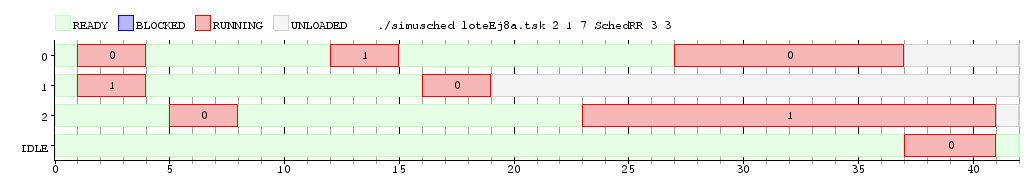
\includegraphics[scale=0.45]{../tp1/Test/resEj8Co2SBRRMM.png}
\\
\vspace{1pt}
\footnotesize\textit{Simulacro RR con 2 n\'ucleos de quantum 3.\\Con 7 ticks de costo de migraci\'on.}
\end{center}
\vspace{\baselineskip}

\vspace{\baselineskip}
\begin{center}
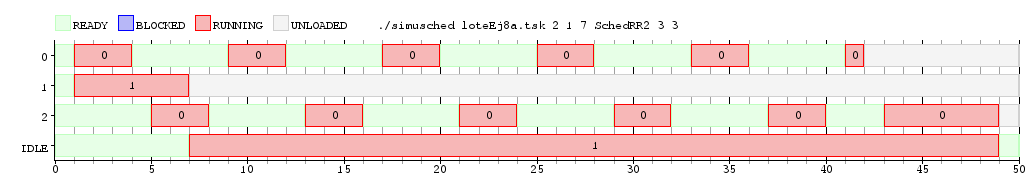
\includegraphics[scale=0.45]{../tp1/Test/resEj8Co2SBRR2MM.png}
\\
\vspace{1pt}
\footnotesize\textit{Simulacro RR2 con 2 n\'ucleos de quantum 3.\\Con 7 ticks de costo de migracion.}
\end{center}
\vspace{\baselineskip}

Podemos notar que, si bien la diferencia se redujo, el tiempo total de RR2 sigue siendo mayor que el de RR. Por lo tanto, concluimos en que 
no permitir la migraci\'on entre procesadores resulta en un rendimiento peor que permiti\'endola. Sin embargo, vale la pena notar que nuestra 
experimentaci\'on contempla los casos para los cuales el costo de migrar una tarea de un procesador a otro no es excesivamente mayor al doble
del quantum de los procesadores, y ser\'ia un interesante experimento futuro (que dejamos afuera por lo acotado del tiempo para hacer este informe)
comprobar el comportamiento de estas dos pol\'iticas de scheduling con tiempos de migraci\'on progresivamente mayores, y dejando fijo el quantum
de los procesadores.

\subsection{Ejercicio 9: Prioridades fijas vs Prioridades Din\'amicas}

Para este ejercicio, debimos idear un lote de tareas que cumpliera, en simult\'aneo, las siguientes condiciones:

\begin{itemize}
 \item Tener un scheduling no factible para el algoritmo de prioridades fijas
 \item Tener un scheduling factible para el algoritmo de prioridades din\'amicas
\end{itemize}

El lote que propusimos para este experimento es el siguiente:

\begin{verbatim}
  lote-ej9.tsk:
    &A1,10,4
    &B3,4,1
\end{verbatim}

Es decir, una repetici\'on de tarea de tipo A, con 4 ciclos de clock de tiempo de ejecuci\'on y 10 ciclos de clock como per\'iodo, y 3 repeticiones 
de tareas de tipo B, con 1 ciclo de clock de tiempo de ejecuci\'on y per\'iodo igual a 4. A continuaci\'on, mostraremos que con esta combinaci\'on
de per\'iodos y tiempos de ejecuci\'on, la tarea A no terminar\'a de ejecutarse antes de su \textit{deadline} (ciclo de clock n\'umero 10) 
para el scheduler de prioridades fijas. Es importante notar que a los tiempos de ejecuci\'on de las dos familias de tareas hay que sumarle el ciclo
de clock extra correspondiente a la llamada a \textit{exit()}. Por lo tanto, la tarea A requerir\'a de 5 ciclos para completar su ejecuci\'on, y las tareas 
B requerir\'an de 2 ciclos cada una. 
\\
El raz\'onamiento que nos llev\'o a elegir este lote de tareas para este ejercicio fue el siguiente: si una tarea con una per\'iodo muy largo respecto
de la cantidad de ciclos de clock necesaria para su ejecuci\'on (en nuestro ejemplo, esta tarea es la A) es continuamente interrumpida por muchas 
solicitudes para ejecutar tareas de per\'iodo muy corto (las B, en nuestro ejemplo), el scheduler de prioridades fijas siempre elegir\'ia a las de 
per\'iodo corto, mientras que el de prioridades din\'amicas tomar\'ia en cuenta cu\'anto falta para que haya un \textit{overflow} causado por la tarea de
per\'iodo largo y, estando cerca de la deadline de dicha tarea, le dar\'ia, finalmente, el uso del procesador para que pueda terminar su ejecuci\'on.

Veamos el diagrama de Gantt para este lote, con scheduling con prioridades fijas:

\vspace{\baselineskip}
\begin{center}
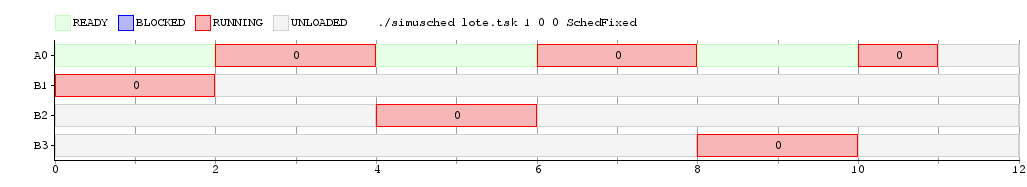
\includegraphics[scale=0.45]{../tp1/Test/ejercicio9-1.png}
\\
\vspace{1pt}
\footnotesize\textit{Simulaci\'on SchedFixed}
\end{center}
\vspace{\baselineskip}

En los instantes m\'ultiplos de 4 (0, 4 y 8) llega al sistema una \textit{request} por una tarea de familia B, mientras que en el instante 0 llega la \'unica 
\textit{request} por una tarea de tipo A. Como las tareas de tipo B, por tener menor per\'iodo, son m\'as prioritarias que la de tipo A, en los instantes
0, 4 y 8, el scheduler decide poner a correr las tareas de tipo B, durante los dos ciclos que necesitan para terminar. Esto le deja a la tarea A
4 ciclos de clock disponibles en los primeros 10 ciclos de clock, con lo cual no puede terminar la ejecuci\'on antes de que llegue su deadline,
haciendo inviable el uso del scheduler de prioridades fijas para este lote de tareas.
\\
Ejecutando el mismo lote de tareas, pero con scheduling de prioridades din\'amicas, obtenemos el siguiente diagrama de Gantt:

\vspace{\baselineskip}
\begin{center}
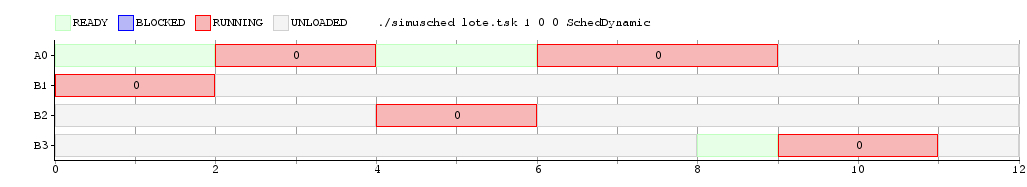
\includegraphics[scale=0.45]{../tp1/Test/ejercicio9-2.png}
\\
\vspace{1pt}
\footnotesize\textit{Simulaci\'on SchedDynamic}
\end{center}
\vspace{\baselineskip}

En esta simulaci\'on, el comportamiento del scheduler es id\'entico al de prioridades fijas hasta el instante 8, correspondiente a la tercer \textit{request}
por una tarea de tipo B. En este instante, la tarea de tipo A tiene su deadline dentro de 2 ciclos de clock, mientras que la tarea de tipo B tiene
su deadline a 4 ciclos de clock de distancia, por lo cual el scheduler decidir\'a poner a correr a la tarea de tipo A en vez de la tarea de tipo B.
Esto le permitir\'a a la tarea de tipo A consumir el \'ultimo ciclo de CPU que necesitaba, y luego el scheduler pondr\'a a correr a la \'ultima
tarea de tipo B, que terminar\'a sin problemas su ejecuci\'on. As\'i, todas las tareas del lote terminaron su ejecuci\'on antes de su \textit{deadline}.
Aqu\'i vale la pena notar que, si bien consideramos que era m\'as claro mostrar exactamente en qu\'e punto de la ejecuci\'on (y por qu\'e) difieren las 
pol\'iticas de los dos schedulers utilizados en este ejercicio, era f\'acil verificar que el scheduling con prioridades din\'amicas para este lote era
factible recurriendo al teorema 7 del art\'iculo analizado en el ejercicio 5. En efecto, reemplazando todos los valores en la f\'ormula del teorema:

\begin{equation*}
 C_{1}/T_{1} + C_{2}/T_{2} = (5/10) + (2/4) = 1 \leq 1
\end{equation*}

como quer\'iamos ver.